\selectlanguage{italian}
\graphicspath{ {img/5/} }
\chapter{Realizzazione e sviluppo del software}\label{cap:software}
\thispagestyle{empty} %Elimina il numero della prima pagina del capitolo.
\newpage
\section{L'approccio utilizzato}
\vspace{8mm}
Il software è stato realizzato utilizzando due Haar Cascades attraverso i quali vengono riconosciuti occhi e viso. Gli Haar Cascades utilizzati sono nel formato \ac{XML} e sono distribuiti in maniera \emph{open source} da \emph{Intel Corporation}.
Gli Haar Cascades sono stati utilizzati grazie ai CascadeClassifier forniti all'interno della libreria \emph{OpenCV}.

Il software prodotto, ottenuto attraverso l'impiego del linguaggio di programmazione \emph{Python}, è costituito di due script,  ExtractSector.py e IrisSegmentation.py, che verranno descritti in seguito.
Da un punto di vista ad alto livello, il software ottiene la riproduzione live utilizzando una webcam, tale riproduzione viene analizzata di frame in frame, ogni frame è successivamente portato in grayscale per permettere un'analisi più efficiente.
Una volta fatto ciò, vengono individuati viso, occhi, e iride, e su richiesta dell'utente verrà effettuata la segmentazione, polarizzazione e codifica delle iridi degli occhi.
\begin{figure}[h!]
	\centering
	
\includegraphics[width=120mm]{img/5/intel1.png}
	\caption{\fontsize{10px}{0mm}\selectfont Intel License Agreement\label{fig:intel_1_1}}
\end{figure} \newpage
\begin{figure}[h!]
	\centering
	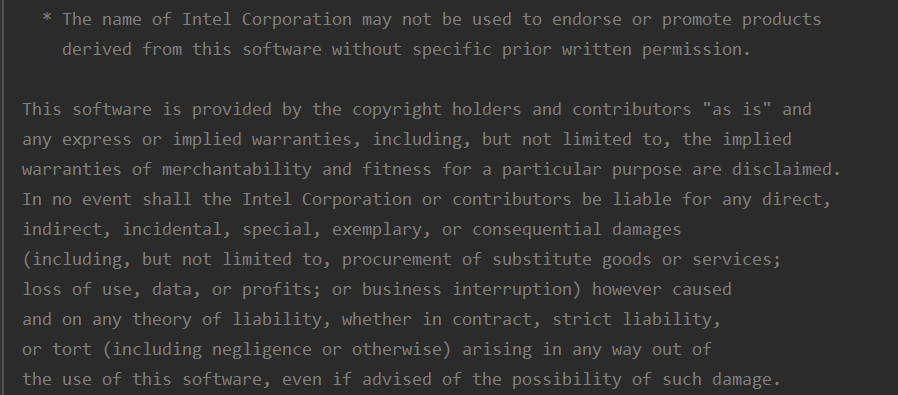
\includegraphics[width=120mm]{img/5/intel2.png}
	\caption{\fontsize{10px}{0mm}\selectfont Intel License Agreement \label{fig:intel_1_2}}
\end{figure}
\newpage
\section{Codice}
\vspace{8mm}
\subsection{Lo script Iris Segmentation}
Iris Segmentation è lo script contenente la maggior parte delle operazioni effettuate dal sistema. Come già accennato precedentemente, vengono utilizzati due Haar Cascades per il riconoscimento di viso e occhi. 
Lo script inizia ottenendo la riproduzione live a partire dalla webcam che verrà mostrata in una finestra, le cui dimensioni sono specificate in riga 12 e 13.

\begin{figure}[h!]
	\centering
	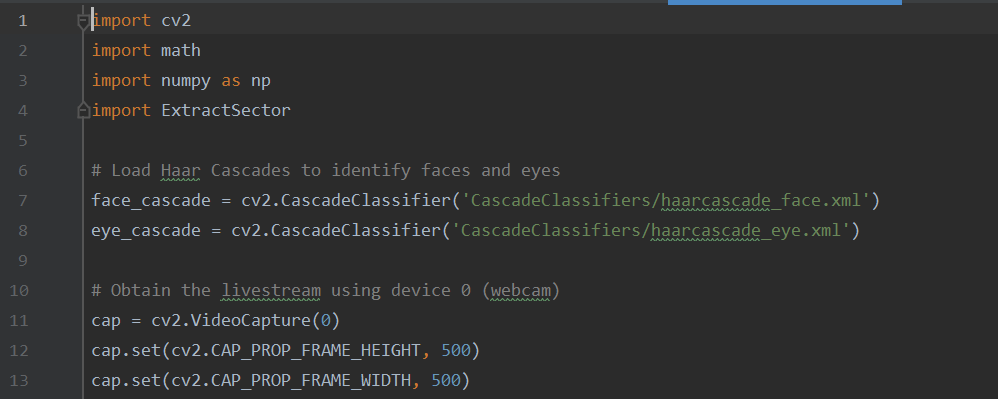
\includegraphics[width=120mm]{img/5/codice_1_1}
	\caption{\fontsize{10px}{0mm}\selectfont Fasi iniziali\label{fig:codice_1_1}}
\end{figure}

Una volta inizializzata la cattura, bisogna prendere le immagini di frame in frame, in un loop infinito, questa operazione viene eseguita attraverso il metodo \emph{read} in riga 17. Come vedremo successivamente, il loop può essere arrestato su input dell'utente.
Ottenute le immagini, introduciamo un concetto chiave, chiamato \emph{roi}, ossia la regione di interesse(region of interest) che viene analizzata in ogni dato istante.
\begin{figure}[h!]
	\centering
	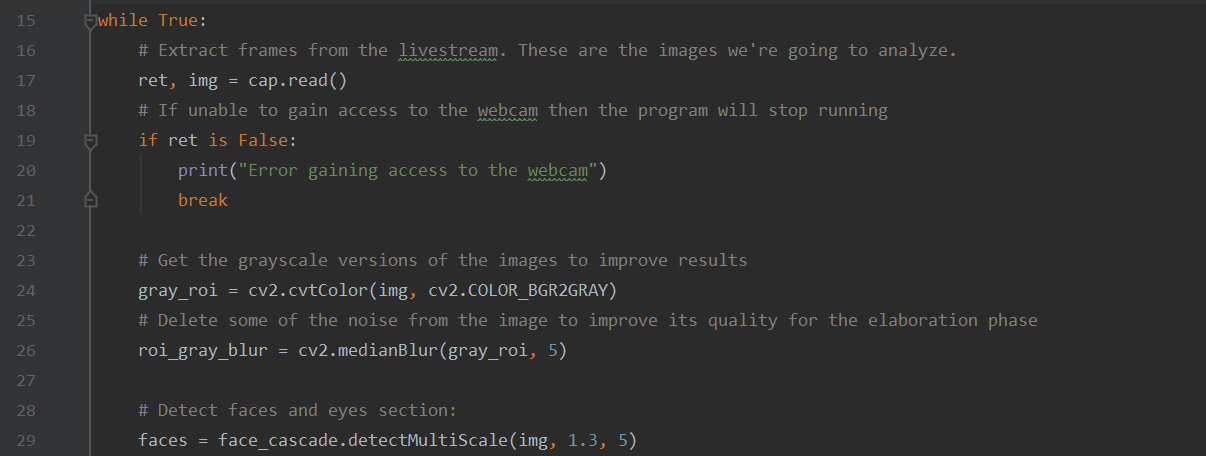
\includegraphics[width=120mm]{img/5/codice_1_2}
	\caption{\fontsize{10px}{0mm}\selectfont Fasi iniziali e processing \label{fig:codice_1_2}}
\end{figure}\newpage

La regione di interesse, inizialmente, corrisponde all'intera immagine, che verrà convertita in grayscale per risultati più precisi. In seguito, attraverso l'utilizzo del metodo \emph{medianBlur} cancelleremo parte del noise contenuto all'interno dell'immagine in maniera tale da permette al sistema di lavorare in maniera più efficace durante la fase di elaborazione.
\begin{figure}[h!]
	\centering
	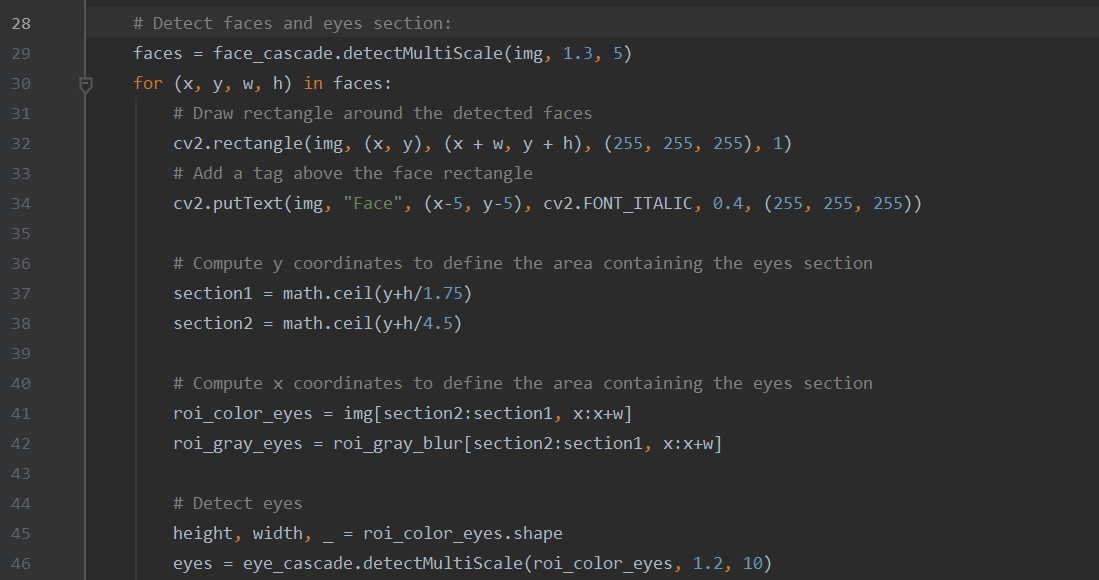
\includegraphics[width=120mm]{img/5/codice_1_3}
	\caption{\fontsize{10px}{0mm}\selectfont Riconoscimento del viso \label{fig:codice_1_3}}
\end{figure}\newline

Una volta terminate le operazioni di processing dell'immagine viene avviata la procedura principale. Essa comincia effettuando una ricerca dei volti all'interno dell'immagine considerata nel dato istante, nel caso positivo, ossia quando vengono riconosciuti dei volti all'interno dell'immagine, l'algoritmo non fa altro che mostrare all'utente un rettangolo attorno ai volti attraverso la finestra mostrata precedentemente.

Durante la fase di progettazione è stato introdotto un concetto, denominato \emph{fascia degli occhi}, che non è altro che l'area del viso all'interno della quale sono presenti gli occhi. Il software, quindi, una volta rilevati dei volti, calcola la fascia degli occhi, che diventerà la nuova region of interest.
All'interno della nuova region of interest verrà avviata una nuova scansione, in particolare, verranno ricercati gli occhi considerando \textit{unicamente} la nuova immagine la cui area corrisponde alla region of interest. Questa scelta migliora le prestazioni sia in termini di computazione, sia in termini di tempo impiegato.\newpage

In questa sezione di codice viene disegnato un rettangolo attorno ad ogni occhio, in particolare indicando precisamente l'occhio sinistro e l'occhio destro.

Arrivati a questo punto, è stata completata la fase iniziale di riconoscimento del viso e degli occhi.
\begin{figure}[h!]
	\centering
	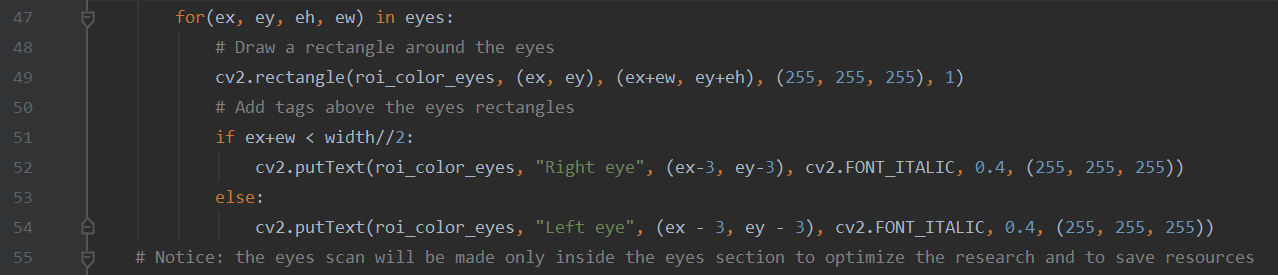
\includegraphics[width=120mm]{img/5/codice_1_4}
	\caption{\fontsize{10px}{0mm}\selectfont Riconoscimento degli occhi \label{fig:codice_1_4}}
\end{figure}

Viene mostrata una finestra contenente la cattura live e le informazioni minimali per l'utilizzo del software.
Grazie alle procedure indicate precedentemente, quando verrà riconosciuto un volto verrà disegnato un rettangolo attorno ad esso, stesso procedimento per gli occhi.

\begin{figure}[h!]
	\centering
	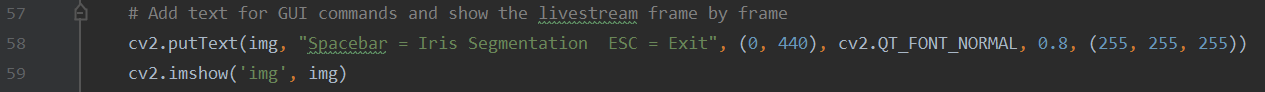
\includegraphics[width=120mm]{img/5/codice_1_5}
	\caption{\fontsize{10px}{0mm}\selectfont Completamento GUI \label{fig:codice_1_5}}
\end{figure}

Arrivati a questo punto, utilizziamo una variabile $$k$$ per catturare gli input dell'utente, in base al tipo di tasto premuto, verrà effettuata un'azione. Quando viene premuto il tasto ESC verrà chiuso il programma.

\begin{figure}[h!]
	\centering
	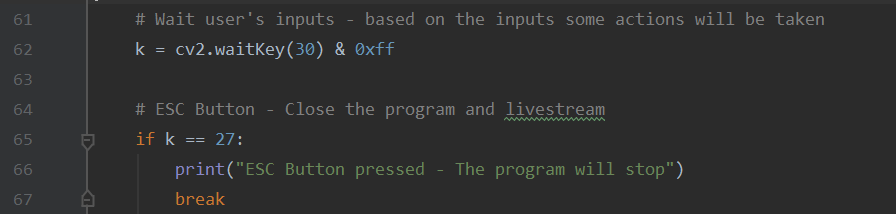
\includegraphics[width=120mm]{img/5/codice_1_6}
	\caption{\fontsize{10px}{0mm}\selectfont Input utente \label{fig:codice_1_6}}
\end{figure}
\newpage
Di seguito è riportata la procedura di segmentazione e codifica dell'iride. Per avviare la procedura l'utente dovrà premere il tasto spacebar, come indicato sulla \ac{GUI}.
Viene utilizzato il metodo \emph{HoughCircles} per permettere l'identificazione della pupilla e della sclera.\footnote{La sclera è la membrana bianca attorno all'occhio}
L'idea è la seguente: una volta individuate le pupille e le sclere, attraverso l'utilizzo di una flag per distinguere l'occhio considerato, viene effettuata la segmentazione delle iridi, in particolare verranno salvate due immagini distinte, una per occhio, contenenti appunto i due occhi. Queste immagini verranno utilizzate in seguito.
Per motivi di design, vengono salvate anche tutte le immagini ottenute durante il processing e durante l'esecuzione del software.
\begin{figure}[h!]
	\centering
	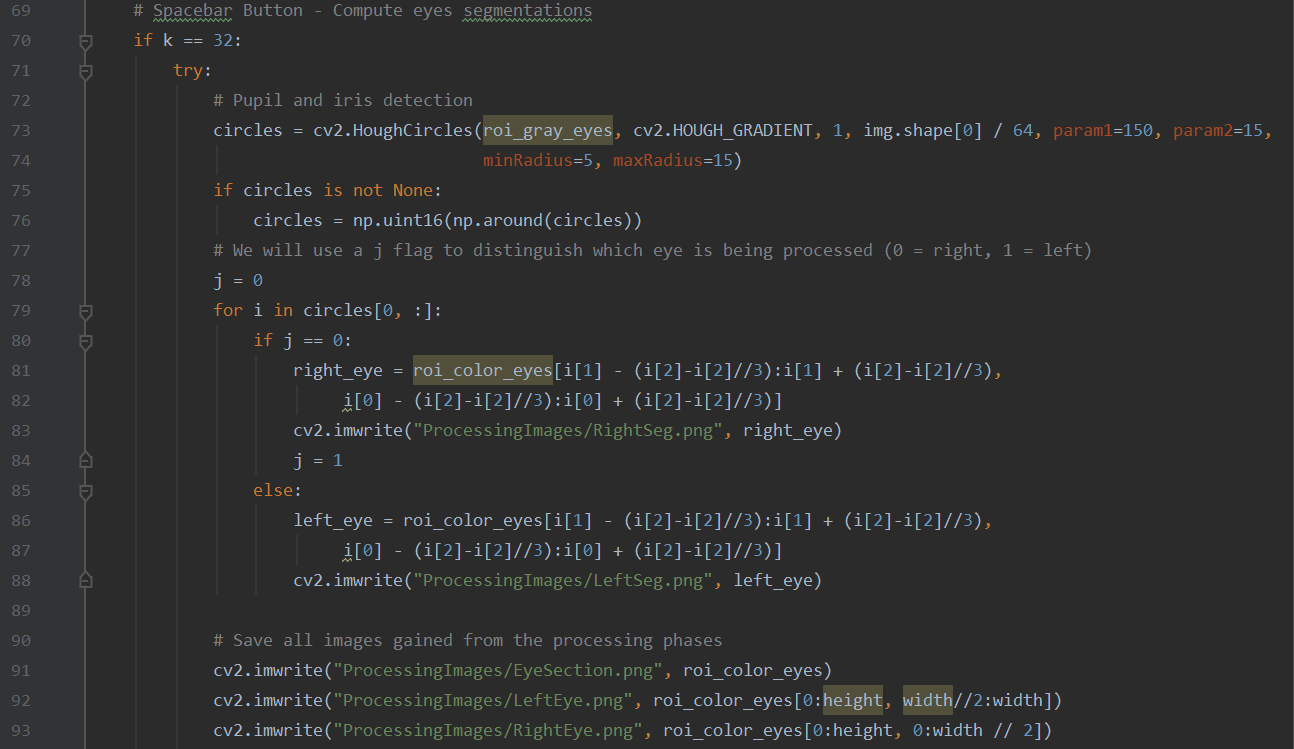
\includegraphics[width=120mm]{img/5/codice_1_7}
	\caption{\fontsize{10px}{0mm}\selectfont Segmentazione dell'iride \label{fig:codice_1_7}}
\end{figure}
L'ultima sezione di codice mostra la fase di chiusura della cattura e il rilascio della webcam, precedute dal metodo segmentation dello script Extract Sector, descritto in seguito. 
\begin{figure}[h!]
	\centering
	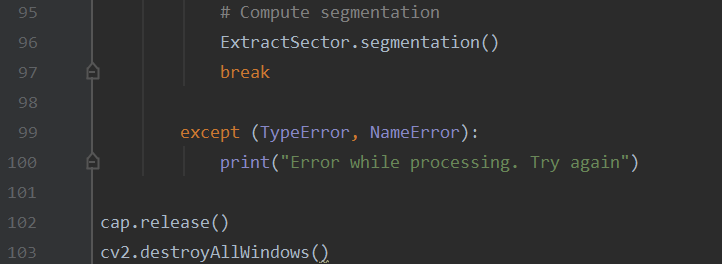
\includegraphics[width=120mm]{img/5/codice_1_8}
	\caption{\fontsize{10px}{0mm}\selectfont Segmentazione dell'iride e Extract Sector \label{fig:codice_1_8}}
\end{figure}\newpage

\subsection{Lo script Extract Sector}
Lo script Extract Sector svolge la fase finale, al fine della quale vengono ottenute le codifiche delle due iridi degli occhi.
In particolare, viene utilizzato \emph{image slicer} per sezionare l'iride considerata, dopodichè viene effettuata la polarizzazione a partire dalle stesse immagini, e infine la codifica.
\begin{figure}[h!]
	\centering
	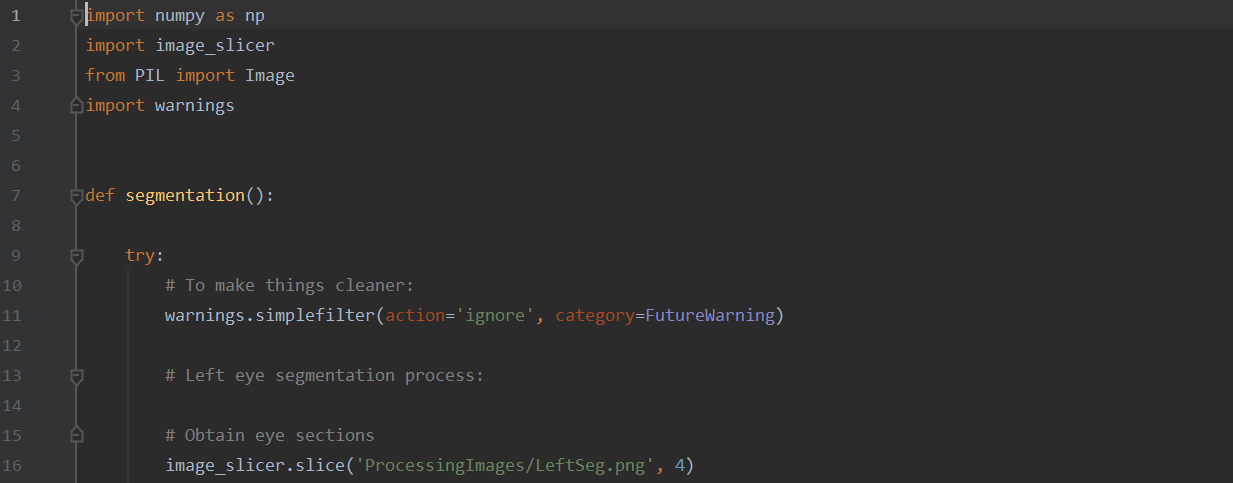
\includegraphics[width=120mm]{img/5/codice_1_9}
	\caption{\fontsize{10px}{0mm}\selectfont Il metodo segmentation \label{fig:codice_1_9}}
\end{figure}
La procedura è identica per entrambi gli occhi. Si inizia ottenendo le quattro sezioni dell'iride e scalandole tutte alla stessa grandezza(in particolare la grandezza della più piccola sezione per evitare di danneggiare l'output finale).
Una volta ottenute le sezioni, si esegue la polarizzazione unendo le immagini in un'unica immagine, sulla quale viene eseguita la codifica.\newpage
\begin{figure}[h!]
	\centering
	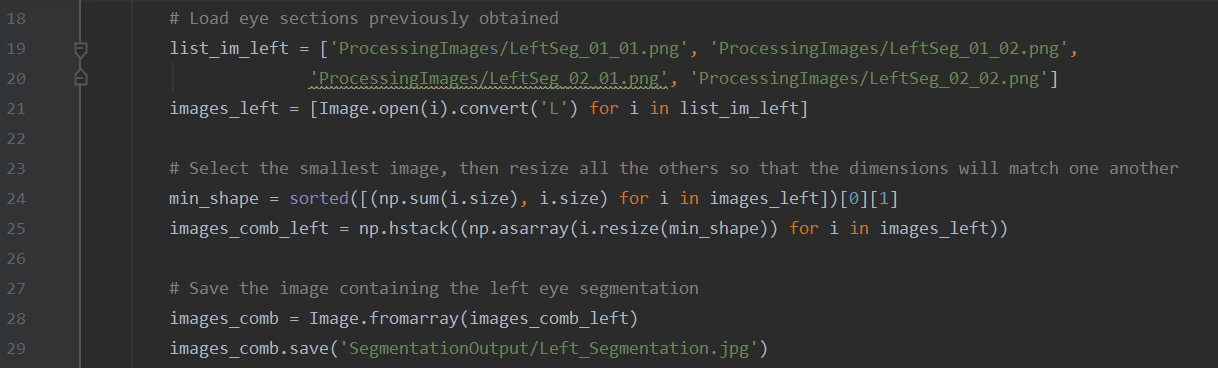
\includegraphics[width=120mm]{img/5/codice_1_10}
	\caption{\fontsize{10px}{0mm}\selectfont Occhio sinistro \label{fig:codice_1_10}}
\end{figure}

\begin{figure}[h!]
	\centering
	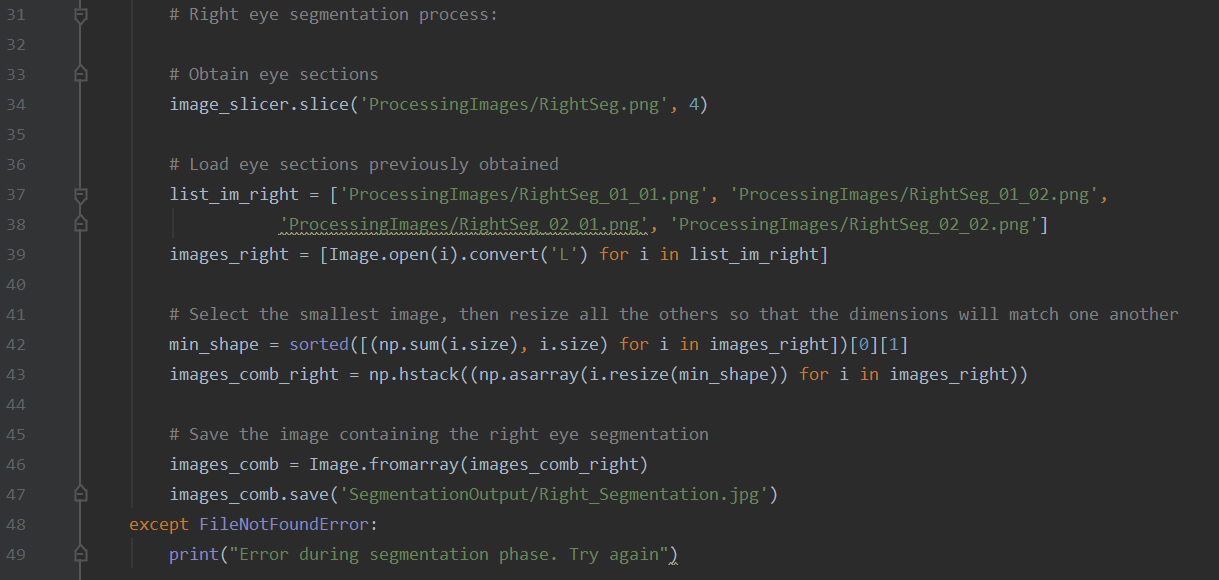
\includegraphics[width=120mm]{img/5/codice_1_11}
	\caption{\fontsize{10px}{0mm}\selectfont Occhio destro \label{fig:codice_1_11}}
\end{figure}
\newpage